\documentclass{article}

\usepackage[english]{babel}
\usepackage[letterpaper,top=2cm,bottom=2cm,left=3cm,right=3cm,marginparwidth=1.75cm]{geometry}

% Useful packages
\usepackage{amsmath}
\usepackage{graphicx}
\usepackage[colorlinks=true, allcolors=blue]{hyperref}

\title{Tema Practica ML}
\author{Al Ihtiar Peter \\ Cobaschi Emanuel-Aser\\  Grupa A1}

\begin{document}
\maketitle

\section{Introducere}
In rezolvarea acestei teme practice, am implementat algoritmii Bayes-Naive si K-NN, facand o comparatie intre ei. De asemenea, fiecare este comparat cu metodele clasice si banale: datul cu banul si alegerea mereu a aceluiasi raspuns(non-spam). Pentru partea de bonus, am implementat tot o varianta de Bayes-Naive, aspectele legate de preprocesari si rezultatele fiind descrise in cele ce urmeaza. Pentru fiecare algoritm este analizat si comportamentul la Cross-Validation Leave-One-Out.

\section{Bayes-Naive}
Am ales sa implementam algoritmul Bayes-Naive, acesta fiind in general ales pentru clasificarea mesajelor, datorita performantei sale bune in contextul analizei textelor si eficientei in gestionarea seturilor mari de date. De asemenea, a dat rezultate mai bune decat KNN.
\subsection{Preprocesarea datelor}
In cazul de baza al problemei, testarea se face pe directoarele intitulate cu 'part10', toate celelalte fiind folosite la partea de antrenare. \\
Atributele sunt cuvintele din fiecare mesaj, iar eticheta este 1(spam) sau 0(not-spam), data de aparitia sau nu in numele fisierului a secventei 'spm'.\\ In acest sens, fiecare mesaj este preprocesat, fiind eliminate semnele de punctuatie, masjusculele si celelalte caractere speciale, obtinandu-se o lista de cuvinte.
\subsection{Antrenare}
Pe baza datelor de antrenament sunt calculate asadar probabilitatile ca mesajul sa fie catalogat ca spam si not-spam, iar pentru fiecare cuvant din vocabularul folosit, se calculeaza de asemenea probabilitatile aparitiei acestuia, in functie de valoarea etichetei.\\
\subsection{Testare}
Pentru fiecare mesaj din setul de date de testare, in care atributele de intrare sunt cuvintele din mesaj, se calculeaza p(spam) si p(not-spam) folosind Teorema lui Bayes si apoi, pe baza rezultatului mai mare, se face predictia. \\
\subsection{Rezultate}
    Comparand algoritmul Bayes-Naive implementat cu metodele banale : datul cu banul si obtinerea mereu a valorii 0, se obtin urmatoarele rezultate
    \begin{figure}[ht]
    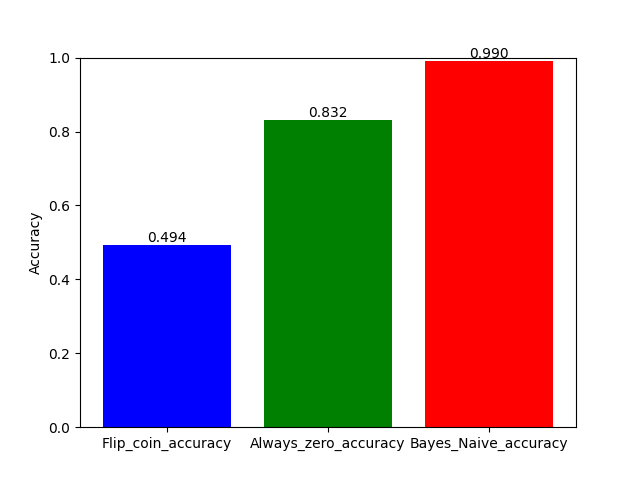
\includegraphics[width=0.8\textwidth]{Figure_1.png}
    \label{fig:result_image}
    \end{figure}

\\


\subsection{CVLOO}
    Pentru algoritmul Bayes-Naive implementat am aplicat strategia Cross Validation Leave-One-Out, in felul urmator: fiecare dintre \{'part1', 'part2', \dots , 'part10'\} a devenit pe rand subiect de testare, antrenarea facandu-se pe celelalte 9. Au fost obtinute urmatoarele rezultate:
    \newpage
    \begin{figure}[h]
    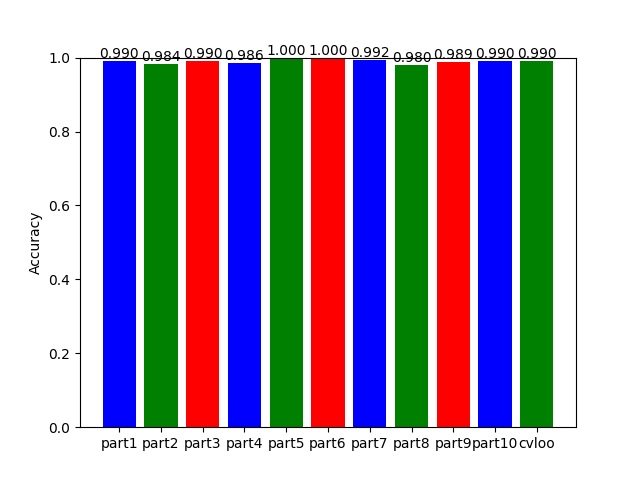
\includegraphics[width=0.8\textwidth]{Bayes_CVLOO.png}
    \label{fig:bayes_cvloo}
    \end{figure}


\section{K-NN}
Am ales sa implementam algoritmul K-NN, acesta fiind un algoritm relativ usor de implementat, care nu necesita antrenare, si care functioneaza bine pentru date cu zgomot. Totodata, am implementat acest algoritm cu scopul compararii cu Bayes-Naive.
\subsection{Preprocesarea datelor}
In cazul de baza al problemei, testarea se face pe directoarele intitulate cu 'part10', toate celelalte fiind folosite la partea de antrenare. \\
Atributele sunt cuvintele din fiecare mesaj, iar eticheta este 1(spam) sau 0(not-spam), data de aparitia sau nu in numele fisierului a secventei 'spm'.\\
Totusi, este necesara introducerea unei notiuni noi, si anume o metoda de a calcula distantele dintre instante. In acest sens, folosim distanta Levenshtein, metoda uzuala in prelucrarea textelor. Astfel, pentru doua instante oarecare, se preproceseaza mesajul lor, fiind eliminate semnele de punctuatie, masjusculele si celelalte caractere speciale. Asupra listelor de cuvinte obtiune se aplica distanta Levenshtein si rezultatul reprezinta distanta cu care va lucra algoritmul K-NN dintre cele doua instante.
\subsection{Testare}
Pentru fiecare mesaj din setul de date de testare, se calculeaza distanta fata de toate mesajele din setul de antrenament. Predictia va fi votul majoritar al celor mai apropiate K instante din setul de antrenament.
\subsection{Rezultate}
    Mentionam ca un aspect crucial in acest algoritm este determinarea unui K cat mai favorabil. Noi am lucrat cu K = 1001 si am obtinut urmatoarele rezultate:


    \newpage
    \begin{figure}[ht]
    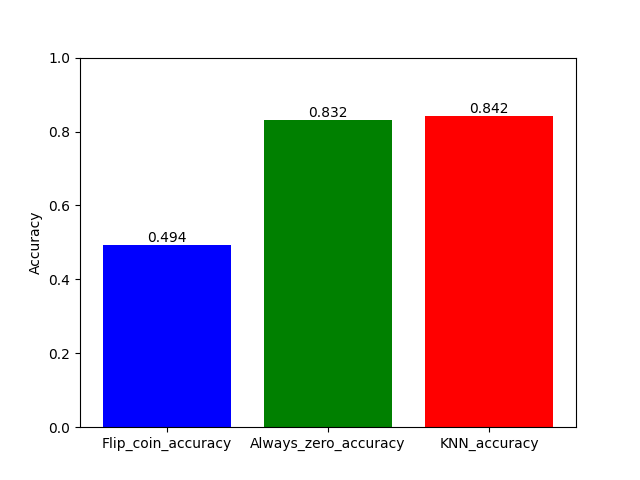
\includegraphics[width=0.8\textwidth]{Figure_2.png}
    \label{fig:result_image}
    \end{figure}


\subsection{CVLOO}
    Pentru algoritmul K-NN implementat am aplicat strategia Cross Validation Leave-One-Out, in felul urmator: fiecare dintre \{'part1', 'part2', \dots , 'part10'\} a devenit pe rand subiect de testare, iar setul de antrebare fiind format din celelalte 9. Au fost obtinute urmatoarele rezultate:
    \newpage
    \begin{figure}[ht]
    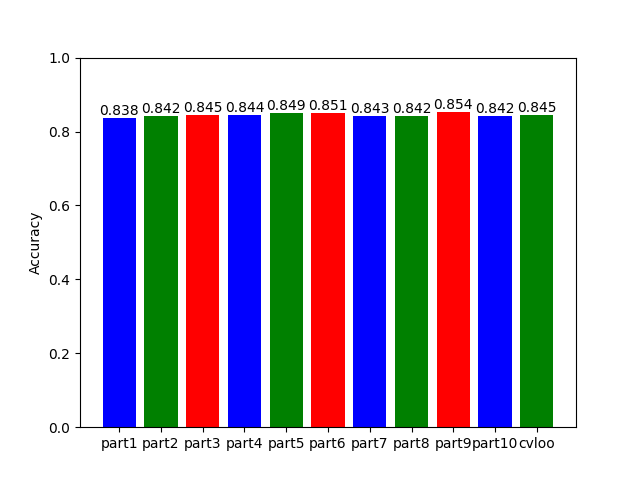
\includegraphics[width=0.8\textwidth]{KNN.png}
    \label{fig:result_image}
    \end{figure}

\section{ Bayes-Naive vs. K-NN}
    Analizand datele din graficele de mai sus, este usor de dedus ca algoritmul Bayes-Naive obtine rezultate mai bune decat K-NN.
    Totusi, pentru claritate, am rezumat aceasta comparatie sub forma urmatorului grafic:
    \newpage
    \begin{figure}[ht]
    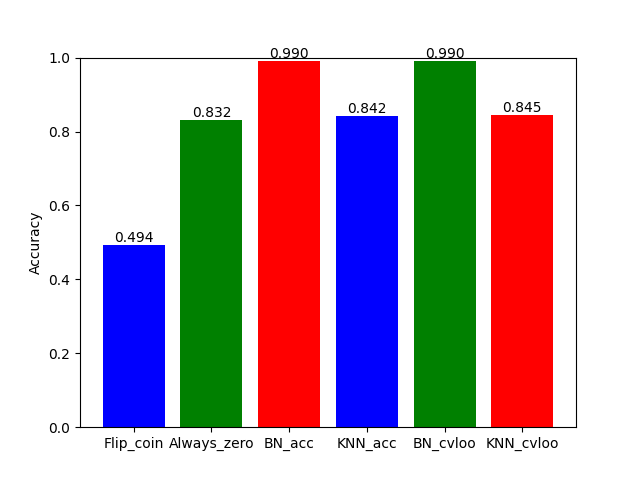
\includegraphics[width=0.8\textwidth]{Bayes_Naive_VS_KNN.png}
    \label{fig:result_image}
    \end{figure}

\section{BONUS}
Pentru partea de Bonus, implementarea este asemanatoare cu cea de la Bayes-Naive descrisa mai sus.
\subsection{Preprocesarea datelor}
Preprocesarea este identica cu cea descrisa mai sus la Bayes-Naive, singura diferenta fiind faptul ca acum avem 3 etichete posibile. Astfel,
atributele sunt cuvintele din fiecare mesaj, iar eticheta este 0(not-spam),
1(spam) sau 2(neetichetat). Evident, conform enuntului de la bonus, toate fisierele din 'part1' si 'part2' vor avea eticheta 2, in timp ce pentru fisierele din \{'part3', 'part4',\dots , 'part10' \} , eticheta este data de aparitia sau nu in numele fisierului a secventei 'spm'.\\ In acest sens, fiecare mesaj este preprocesat, fiind eliminate semnele de punctuatie, masjusculele si celelalte caractere speciale, obtinandu-se o lista de cuvinte.
\subsection{Antrenare}
Pe baza datelor de antrenament sunt calculate asadar probabilitatile ca mesajul sa fie catalogat ca spam si not-spam si neetichetat, iar pentru fiecare cuvant din vocabularul folosit, se calculeaza de asemenea probabilitatile aparitiei acestuia, in functie de valoarea etichetei.\\
\subsection{Testare}
Pentru fiecare mesaj din setul de date de testare, in care atributele de intrare sunt cuvintele din mesaj, se calculeaza p(spam), p(not-spam) si p(neetichetat) folosind Teorema lui Bayes si apoi, pe baza rezultatului mai mare, se face predictia. Acuratetea se calculeaza doar pentru fisierele clasificate drept spam sau non-spam.\\
\subsection{Rezultate}
    Comparand algoritmul de tip Bayes-Naive de la bonus cu metodele banale : datul cu banul si obtinerea mereu a valorii 0, se obtin urmatoarele rezultate
    \begin{figure}[ht]
    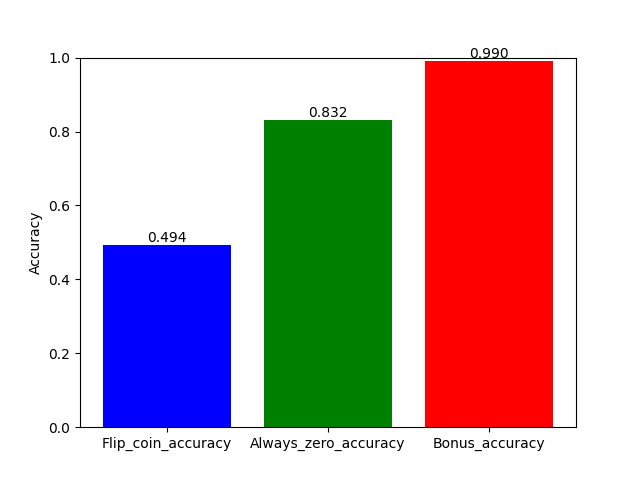
\includegraphics[width=0.8\textwidth]{Figure_3.png}
    \label{fig:result_image}
    \end{figure}
\\


\subsection{CVLOO}
    Pentru algoritmul Bayes-Naive implementat la Bonus am aplicat strategia Cross Validation Leave-One-Out, in felul urmator:  'part1' si 'part2' raman mereu neetichetate si apoi fiecare dintre \{'part3', 'part4', \dots , 'part10'\} a devenit pe rand subiect de testare, antrenarea facandu-se pe celelalte 9. Au fost obtinute urmatoarele rezultate:
    \newpage
    \begin{figure}[ht]
    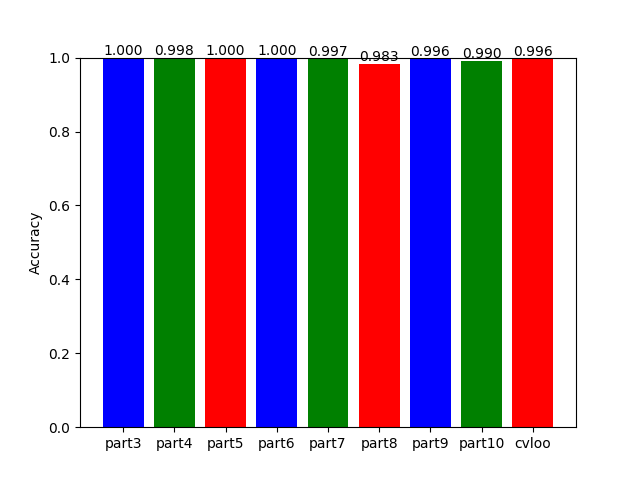
\includegraphics[width=0.8\textwidth]{Bonus_CVLOO.png}
    \label{fig:result_image}
    \end{figure}

\end{document}